\documentclass[a4paper,12pt]{article}
%\documentclass[doc]{apa}
\usepackage[usenames,dvipsnames]{color}
\usepackage{graphicx}
\usepackage{multicol}
\usepackage{multirow}
\usepackage{amsmath}
\usepackage{hyperref}
\usepackage{pdfpages}

%\setlength\parindent{0pt}
%\usepackage{figure}
\usepackage[margin=0.8in]{geometry}
\title{Project 2 Content Based Image Retrieval Using Global and Local Features}
\author{Daniel Bryan and Olmo Zavala\\Florida State University}

\begin{document}
\maketitle

\subsection{Matlab interface}
We created a useful interface to define the corresponding points between two images.
Figure \ref{fig:demo} shows a screenshot of this interface. The user needs to select
corresponding points between images and it doesn't have to be in order (one point in one
image and the next point in the following image). The interface also provides a button to
reset all the points as well as to remove the last added point. These two buttons are
very handy when selecting points. Once all the desired buttons have been selected the 
resulting points are saved in at matlab file that can be stored for later compuatation
using the 8-point algorithm. 

\begin{figure}[h]
    \centering
    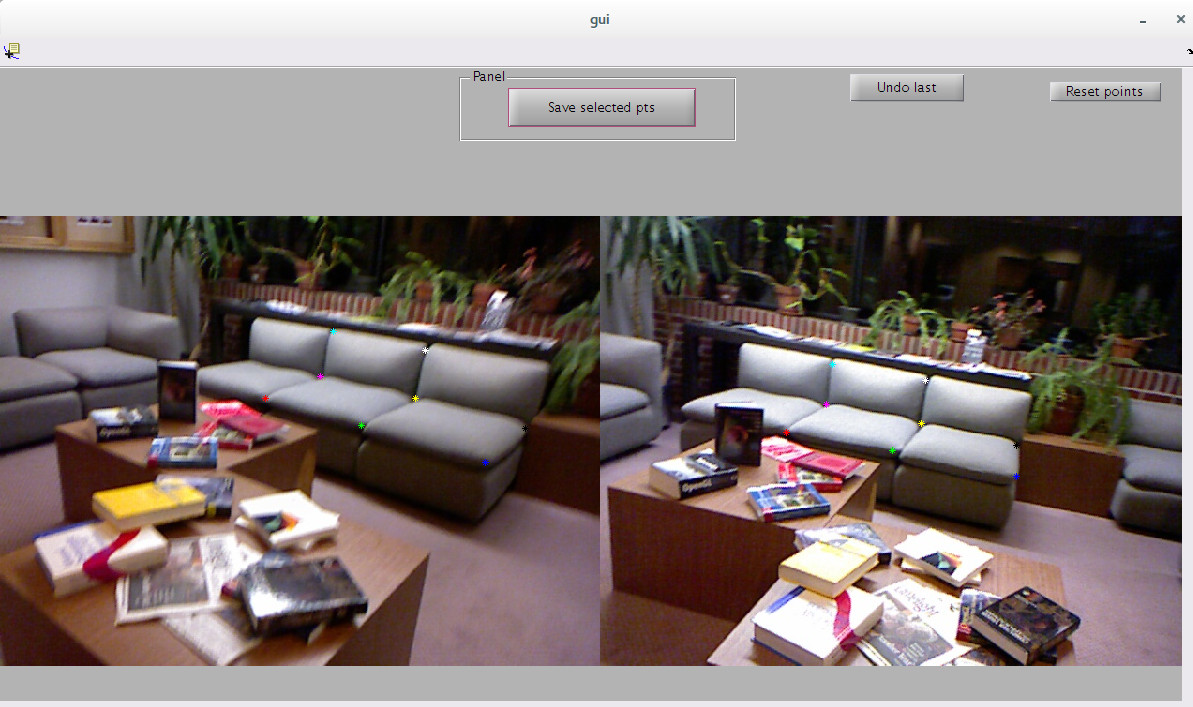
\includegraphics[totalheight=.38\textheight]{./images/Example.jpg}
    \caption{Matlab interface to select corresponding points between two images.
    Example of selecting 9 points using the Matlab interface.}
    \label{fig:demo}
\end{figure}

Each corresponding point is displayed with the same color, 
this makes it easy to see wich points correspond in both of the images.
The coordinates obtained from the selection of points displayed at figure \ref{fig:demo} 
are displayed in figure \ref{fig:pts}.

\begin{figure}[h]
    \centering
    \includegraphics[totalheight=.38\textheight]{./images/pts.png}
    \caption{Obtained coordinates from the selected in figure \ref{fig:demo}.}
    \label{fig:pts}
\end{figure}

In our results we use the example provided by the professor to compare the results. \\

In order to test the correct correspondence of the points obtained by the Matlab interface
we selected 4-points close to the corners of the two figures as displayed in figure \ref{fig:check} 

\begin{figure}[h]
    \centering
    \includegraphics[totalheight=.38\textheight]{./images/Check.jpg}
    \caption{}
    \label{fig:check}
\end{figure}

\subsection{Eight-point algorithm}
\begin{itemize}
    \item Normalize image points
        \begin{itemize}
            \item \textbf{Centroid is at the origin}. We create the matrix $T_{trans}$ for each
                camera like this:
                \begin{equation}
                    \left [
                    \begin{array}[ ]{c c c}
                        1 & 0 & -\mu_x\\
                        0 & 1 & -\mu_y\\
                        0 & 0 & 1\\
                    \end{array}
                \right ]
                \end{equation}
                And we multiply each point of the cameras to they corresponding $T$ matrix like this:
                $Tx_i$.
            \item \textbf{RMS distance from the origin is $\sqrt{2}$.} First compute the RMS of the
                available points:
                \begin{equation}
                    \sqrt{ \frac{1}{n} \sum_{i=1}^n \left(  (x_i - \mu_x)^2 + (y_i- \mu_y)^2) \right) }
                \end{equation}
                Then create $T_{scale}$ and multiply it to each point in the camera. T is:
                \begin{equation}
                    T_s = \left[ 
                    \begin{array}[]{ccc}
                        \sqrt{2}/RMS & 0 & 0 \\
                        0 & \sqrt{2}/RMS  & 0 \\
                        0 & 0 & 1 
                    \end{array}
                     \right]
                \end{equation}
        \end{itemize}
    \item \textbf{Multiply each point by $T_n = T_sT_t$ like this $[u~ v~ 1]' = T_nx$. Do it for each camera.}
    \item \textbf{Solve $x'_nFx_n = 0$ }. To do this we need to form the system $Af = 0$ and solve for f.
        The matrix A is: \begin{equation}
            A = \left[ 
            \begin{array}[ ]{ccccccccc}
                u'_1u_1 & u'_1v_1 & u'_1 & v'_1u_1 &v'_1v_1 & v'_1 & u_1 & v_1 & 1 \\
                u'_2u_2 & u'_2v_2 & u'_2 & v'_2u_2 &v'_2v_2 & v'_2 & u_2 & v_2 & 1 \\
                u'_3u_3 & u'_3v_3 & u'_3 & v'_3u_3 &v'_3v_3 & v'_3 & u_3 & v_3 & 1 \\
                &&& \vdots \\
                u'_nu_n & u'_nv_n & u'_n & v'_nu_n &v'_nv_n & v'_n & u_n & v_n & 1 
            \end{array}
            \right] F = 0
        \end{equation}
    \item \textbf{Find least square solution of $Af = 0$}. 
        \begin{itemize}
            \item First find SVD of A $USV = A$. 
            \item Choose $F_{Norm}$ to be the last column of V
        \end{itemize}
    \item \textbf{Enforcing Singularity} 
        \begin{itemize}
            \item For $F_{Norm}=USV^T$ 
            \item Set $S_3$=0 for 
            \begin{equation}
                       F_{norm} =U \left[ 
            \begin{array}[]{ccc}
                        S_1 & 0 & 0 \\
                        0 & S_2  & 0 \\
                        0 & 0 & S_3 
                    \end{array}
            \right] V^T
            \end{equation}
        \end{itemize}
    \item \textbf{Denormalisation}
    	\begin{equation}
    	F=T_{NormLeft}*F_{Norm}*T_{NormRight}
    	\end{equation}
    \end{itemize}
 

\section{Description}

\subsection{Color histogram}

\subsection{Computation time}

\section{Results}

\end{document}
